% Options for packages loaded elsewhere
\PassOptionsToPackage{unicode}{hyperref}
\PassOptionsToPackage{hyphens}{url}
%
\documentclass[
]{article}
\usepackage{amsmath,amssymb}
\usepackage{lmodern}
\usepackage{ifxetex,ifluatex}
\ifnum 0\ifxetex 1\fi\ifluatex 1\fi=0 % if pdftex
  \usepackage[T1]{fontenc}
  \usepackage[utf8]{inputenc}
  \usepackage{textcomp} % provide euro and other symbols
\else % if luatex or xetex
  \usepackage{unicode-math}
  \defaultfontfeatures{Scale=MatchLowercase}
  \defaultfontfeatures[\rmfamily]{Ligatures=TeX,Scale=1}
\fi
% Use upquote if available, for straight quotes in verbatim environments
\IfFileExists{upquote.sty}{\usepackage{upquote}}{}
\IfFileExists{microtype.sty}{% use microtype if available
  \usepackage[]{microtype}
  \UseMicrotypeSet[protrusion]{basicmath} % disable protrusion for tt fonts
}{}
\makeatletter
\@ifundefined{KOMAClassName}{% if non-KOMA class
  \IfFileExists{parskip.sty}{%
    \usepackage{parskip}
  }{% else
    \setlength{\parindent}{0pt}
    \setlength{\parskip}{6pt plus 2pt minus 1pt}}
}{% if KOMA class
  \KOMAoptions{parskip=half}}
\makeatother
\usepackage{xcolor}
\IfFileExists{xurl.sty}{\usepackage{xurl}}{} % add URL line breaks if available
\IfFileExists{bookmark.sty}{\usepackage{bookmark}}{\usepackage{hyperref}}
\hypersetup{
  pdftitle={Realized Delay: QuickPay (2009-2012)},
  hidelinks,
  pdfcreator={LaTeX via pandoc}}
\urlstyle{same} % disable monospaced font for URLs
\usepackage[margin=1in]{geometry}
\usepackage{graphicx}
\makeatletter
\def\maxwidth{\ifdim\Gin@nat@width>\linewidth\linewidth\else\Gin@nat@width\fi}
\def\maxheight{\ifdim\Gin@nat@height>\textheight\textheight\else\Gin@nat@height\fi}
\makeatother
% Scale images if necessary, so that they will not overflow the page
% margins by default, and it is still possible to overwrite the defaults
% using explicit options in \includegraphics[width, height, ...]{}
\setkeys{Gin}{width=\maxwidth,height=\maxheight,keepaspectratio}
% Set default figure placement to htbp
\makeatletter
\def\fps@figure{htbp}
\makeatother
\setlength{\emergencystretch}{3em} % prevent overfull lines
\providecommand{\tightlist}{%
  \setlength{\itemsep}{0pt}\setlength{\parskip}{0pt}}
\setcounter{secnumdepth}{5}
\usepackage{booktabs,longtable,dcolumn} \usepackage{multirow,array} \usepackage{wrapfig,float} \floatplacement{figure}{H}
\ifluatex
  \usepackage{selnolig}  % disable illegal ligatures
\fi

\title{Realized Delay: QuickPay (2009-2012)}
\author{}
\date{\vspace{-2.5em}Oct 22, 2021}

\begin{document}
\maketitle

\hypertarget{summary-statistics}{%
\section{Summary Statistics}\label{summary-statistics}}

\begin{itemize}
\tightlist
\item
  Continuous variables winsorized at 5\%
\end{itemize}

\begin{table}[ht]
\centering
\begin{tabular}{rllrrr}
  \hline
 & project\_size & started\_and\_ended & number\_of\_projects & number\_of\_tasks & number\_of\_industries \\ 
  \hline
1 & Small & Before QuickPay & 58212 & 942 &  75 \\ 
  2 & Small & After QuickPay & 43583 & 960 &  78 \\ 
  3 & Large & Before QuickPay & 31597 & 841 &  72 \\ 
  4 & Large & After QuickPay & 24511 & 871 &  72 \\ 
   \hline
\end{tabular}
\end{table}
\begin{table}[ht]
\centering
\begin{tabular}{rllrr}
  \hline
 & project\_size & started\_and\_ended & mean\_initial\_duration & sd\_duration \\ 
  \hline
1 & Small & Before QuickPay & 83.60 & 79.26 \\ 
  2 & Small & After QuickPay & 80.95 & 70.28 \\ 
  3 & Large & Before QuickPay & 92.75 & 93.17 \\ 
  4 & Large & After QuickPay & 85.50 & 81.24 \\ 
   \hline
\end{tabular}
\end{table}
\begin{table}[ht]
\centering
\begin{tabular}{rllrr}
  \hline
 & project\_size & started\_and\_ended & mean\_initial\_budget & sd\_budget \\ 
  \hline
1 & Small & Before QuickPay & 41331.05 & 105409.42 \\ 
  2 & Small & After QuickPay & 42047.20 & 104307.87 \\ 
  3 & Large & Before QuickPay & 100573.87 & 192096.57 \\ 
  4 & Large & After QuickPay & 90413.33 & 177999.26 \\ 
   \hline
\end{tabular}
\end{table}
\begin{table}[ht]
\centering
\begin{tabular}{rllrr}
  \hline
 & project\_size & started\_and\_ended & mean\_realized\_delay & sd\_realized\_delay \\ 
  \hline
1 & Small & Before QuickPay & 3.13 & 15.15 \\ 
  2 & Small & After QuickPay & 3.54 & 15.90 \\ 
  3 & Large & Before QuickPay & 6.18 & 21.22 \\ 
  4 & Large & After QuickPay & 5.97 & 20.50 \\ 
   \hline
\end{tabular}
\end{table}

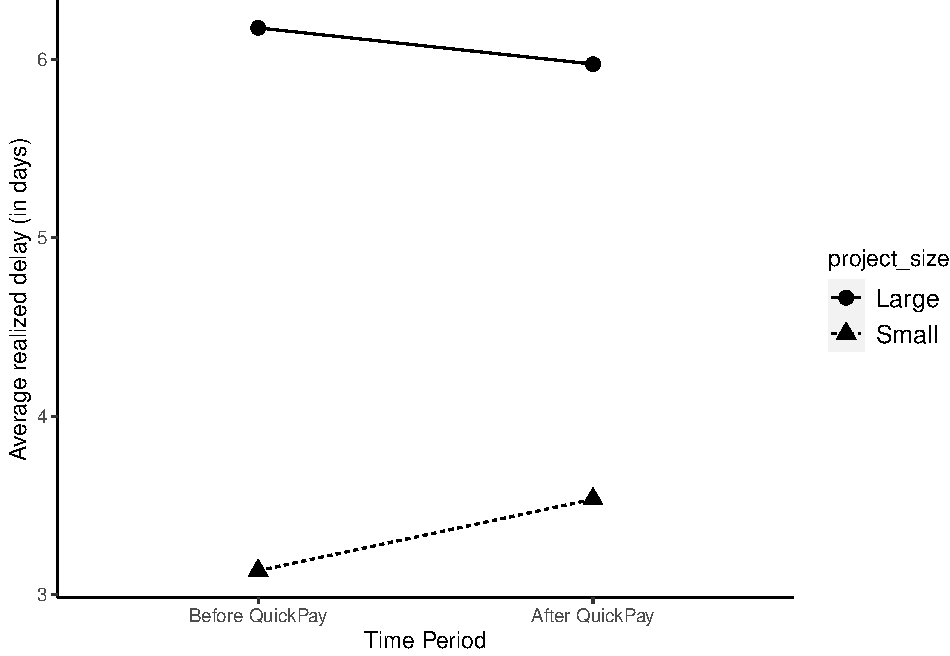
\includegraphics{qp_realized_delay_files/figure-latex/plots-1.pdf}

\hypertarget{linear-regression-full-sample}{%
\section{Linear Regression (Full
Sample)}\label{linear-regression-full-sample}}

\begin{table}[H] \centering 
  \caption{Quickpay 2009-2011} 
  \label{} 
\small 
\begin{tabular}{@{\extracolsep{-2pt}}lcccc} 
\\[-1.8ex]\hline 
\hline \\[-1.8ex] 
\\[-1.8ex] & \multicolumn{4}{c}{$RealizedDelay_{i}$ (in days)} \\ 
\\[-1.8ex] & (1) & (2) & (3) & (4)\\ 
\hline \\[-1.8ex] 
 $Treat_i$ & $-$3.04$^{***}$ & $-$1.97$^{***}$ & $-$1.32$^{***}$ & $-$1.52$^{***}$ \\ 
  & (0.14) & (0.13) & (0.13) & (0.13) \\ 
  & & & & \\ 
 $Post_t$ & $-$0.20 & $-$0.12 & 0.09 & 0.13 \\ 
  & (0.18) & (0.18) & (0.17) & (0.17) \\ 
  & & & & \\ 
 $Treat_i \times Post_t$ & 0.60$^{***}$ & 0.47$^{**}$ & 0.15 & 0.17 \\ 
  & (0.20) & (0.20) & (0.19) & (0.19) \\ 
  & & & & \\ 
 Constant & 6.18$^{***}$ & 5.55$^{***}$ &  &  \\ 
  & (0.12) & (0.13) &  &  \\ 
  & & & & \\ 
\hline \\[-1.8ex] 
Budget, Duration, Bids & No & Yes & Yes & Yes \\ 
Task Fixed Effects & No & No & Yes & Yes \\ 
Naics Fixed Effects & No & No & No & Yes \\ 
Observations & 157,661 & 157,638 & 157,638 & 157,638 \\ 
R$^{2}$ & 0.01 & 0.03 & 0.12 & 0.13 \\ 
Adjusted R$^{2}$ & 0.01 & 0.03 & 0.11 & 0.12 \\ 
\hline 
\hline \\[-1.8ex] 
\textit{Note:}  & \multicolumn{4}{r}{$^{*}$p$<$0.1; $^{**}$p$<$0.05; $^{***}$p$<$0.01} \\ 
 & \multicolumn{4}{r}{SEs are robust and clustered at the project level.} \\ 
\end{tabular} 
\end{table}

\hypertarget{linear-regression-truncated-sample-with-positive-delays}{%
\section{Linear Regression (Truncated Sample with Positive
Delays)}\label{linear-regression-truncated-sample-with-positive-delays}}

\begin{table}[H] \centering 
  \caption{Quickpay 2009-2011 (Truncated with positive delay)} 
  \label{} 
\small 
\begin{tabular}{@{\extracolsep{-2pt}}lcccc} 
\\[-1.8ex]\hline 
\hline \\[-1.8ex] 
\\[-1.8ex] & \multicolumn{4}{c}{$RealizedDelay_{i}$ (in days)} \\ 
\\[-1.8ex] & (1) & (2) & (3) & (4)\\ 
\hline \\[-1.8ex] 
 $Treat_i$ & $-$3.90$^{***}$ & $-$3.03$^{***}$ & $-$3.77$^{***}$ & $-$4.36$^{***}$ \\ 
  & (0.71) & (0.70) & (0.73) & (0.74) \\ 
  & & & & \\ 
 $Post_t$ & $-$2.17$^{***}$ & $-$1.97$^{***}$ & $-$2.05$^{***}$ & $-$1.69$^{**}$ \\ 
  & (0.78) & (0.76) & (0.76) & (0.76) \\ 
  & & & & \\ 
 $Treat_i \times Post_t$ & 2.69$^{**}$ & 2.42$^{**}$ & 1.39 & 1.58 \\ 
  & (1.04) & (1.03) & (1.02) & (1.02) \\ 
  & & & & \\ 
 Constant & 41.51$^{***}$ & 36.69$^{***}$ &  &  \\ 
  & (0.53) & (0.59) &  &  \\ 
  & & & & \\ 
\hline \\[-1.8ex] 
Budget, Duration, Bids & No & Yes & Yes & Yes \\ 
Task Fixed Effects & No & No & Yes & Yes \\ 
Naics Fixed Effects & No & No & No & Yes \\ 
Observations & 18,636 & 18,631 & 18,631 & 18,631 \\ 
R$^{2}$ & 0.002 & 0.04 & 0.21 & 0.23 \\ 
Adjusted R$^{2}$ & 0.002 & 0.04 & 0.17 & 0.19 \\ 
\hline 
\hline \\[-1.8ex] 
\textit{Note:}  & \multicolumn{4}{r}{$^{*}$p$<$0.1; $^{**}$p$<$0.05; $^{***}$p$<$0.01} \\ 
 & \multicolumn{4}{r}{SEs are robust and clustered at the project level.} \\ 
\end{tabular} 
\end{table}

\end{document}
